\section{Module 11. Brain 3D}
\indent
11th module is interactive module, where subsequents steps are conditioned by user action. This is the reason why, the verification of functionality of module included mainly qualitive tests.
Module 11 is displayed in new window. After initialization model of cortex basing on segmentation data is shown. Render window is interactive, user can set camera view by moving computer mouse. It gives possibility to see model from various perspectives (Fig. \ref{fig:figures/11_test_1} - \ref{fig:figures/11_test_2}).  \\


\begin{figure}[H]
\centering{}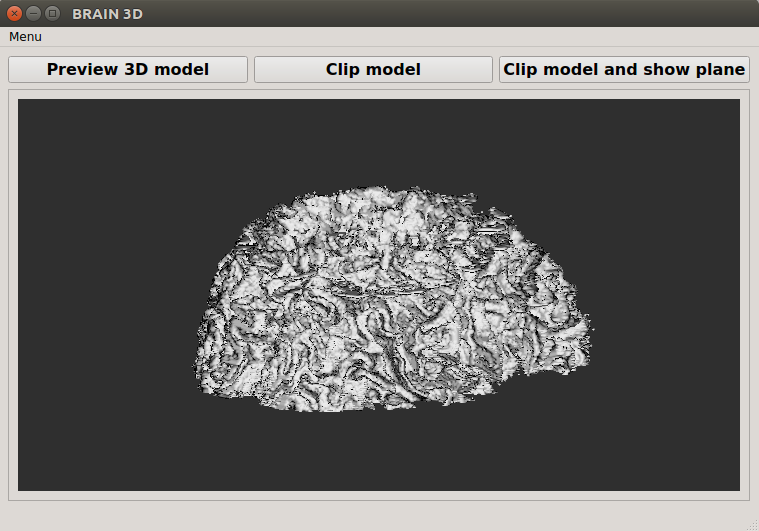
\includegraphics[scale=0.7]{figures/Module_11/11_test_1.png}\caption{Preview model obtained by marching cubes alghoritm. \label{fig:figures/11_test_1}}
\end{figure}


\begin{figure}[H]
\centering{}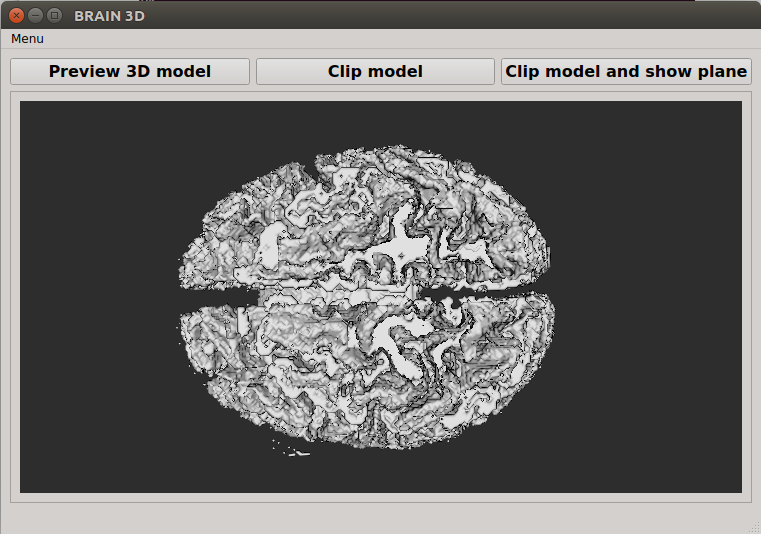
\includegraphics[scale=0.7]{figures/Module_11/11_test_2.png}\caption{Preview model obtained by marching cubes alghoritm. \label{fig:figures/11_test_2}}
\end{figure}

\indent There are three buttons, corresponded to three mode of 11th module. After pressing „Clip model” user can clip model in elected cross-section. To set the intersection plane user has to press middle mouse button. During mouse movement model is automatically clipped.\\

\indent To improve readbility of intersection plane user can display cross-section, by choosing „Clip model and show plane”. In this mode user can also clip model and select plane in the same way as in previous mode.\\
\indent Examples of clipping model in elected cross-section is shown on the figures \ref{fig:figures/11_test_3} - \ref{fig:figures/11_test_8}.

\begin{figure}[H]
\centering{}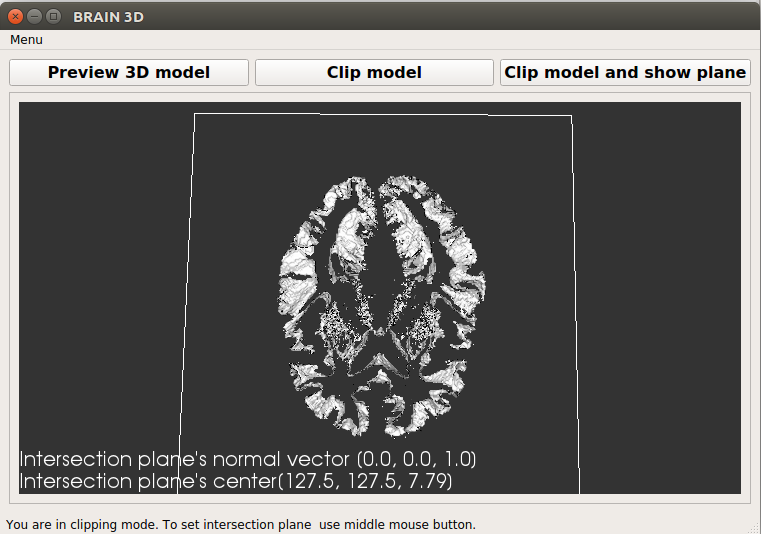
\includegraphics[scale=0.7]{figures/Module_11/11_test_3.png}\caption{Clipped model in transverse plane. \label{fig:figures/11_test_3}}
\end{figure}

\begin{figure}[H]
\centering{}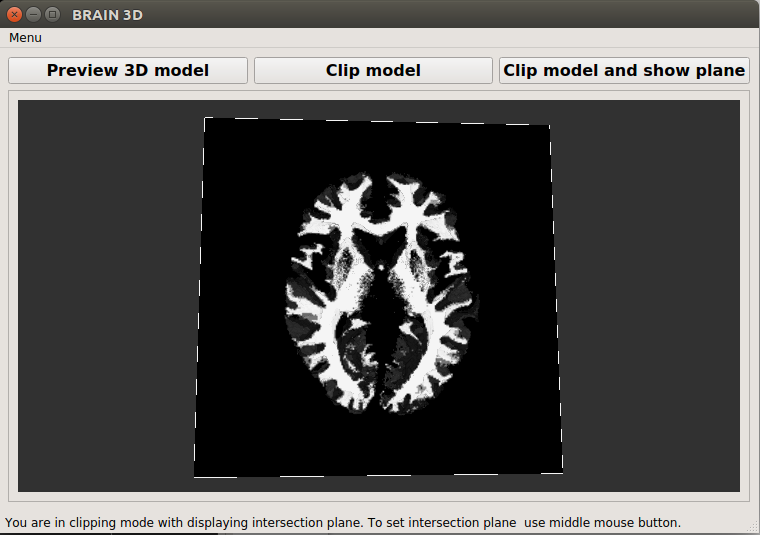
\includegraphics[scale=0.7]{figures/Module_11/11_test_4.png}\caption{Clipped model in the same transverse plane with cross-intersection image. \label{fig:figures/11_test_4}}
\end{figure}

\begin{figure}[H]
\centering{}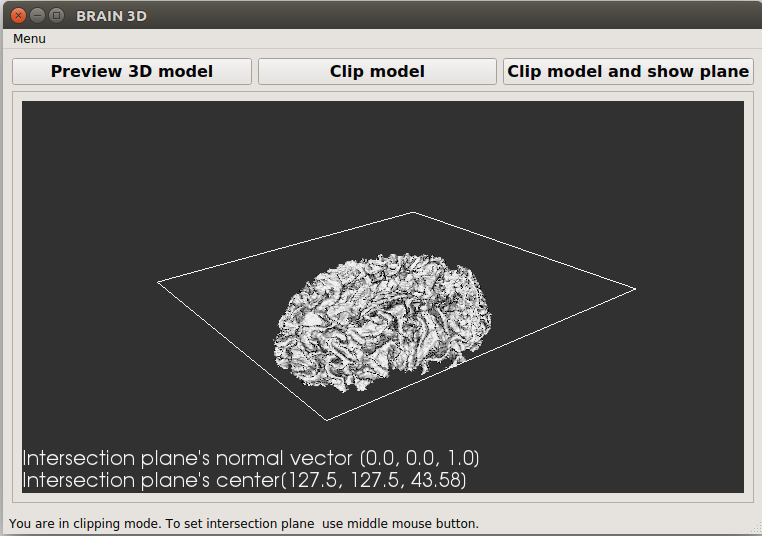
\includegraphics[scale=0.7]{figures/Module_11/11_test_5.png}\caption{Clipped model in transverse plane. \label{fig:figures/11_test_5}}
\end{figure}

\begin{figure}[H]
\centering{}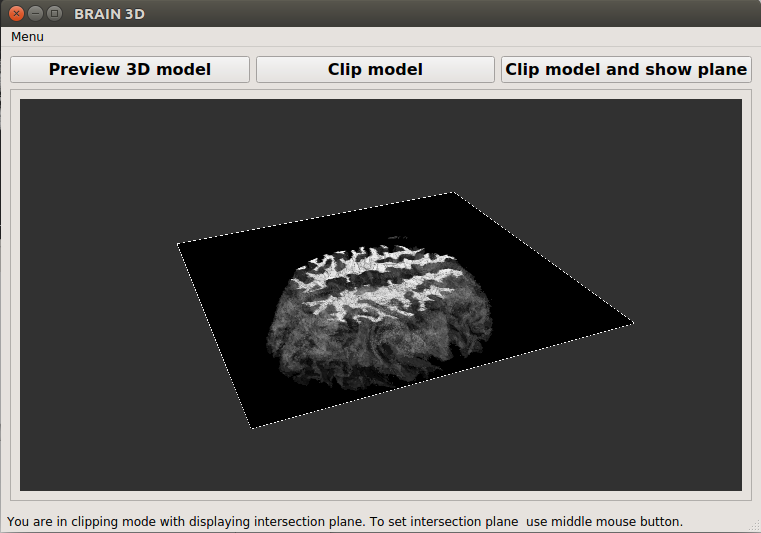
\includegraphics[scale=0.7]{figures/Module_11/11_test_6.png}\caption{Clipped model in the same transverse plane with cross-intersection image. \label{fig:figures/11_test_6}}
\end{figure}


\begin{figure}[H]
\centering{}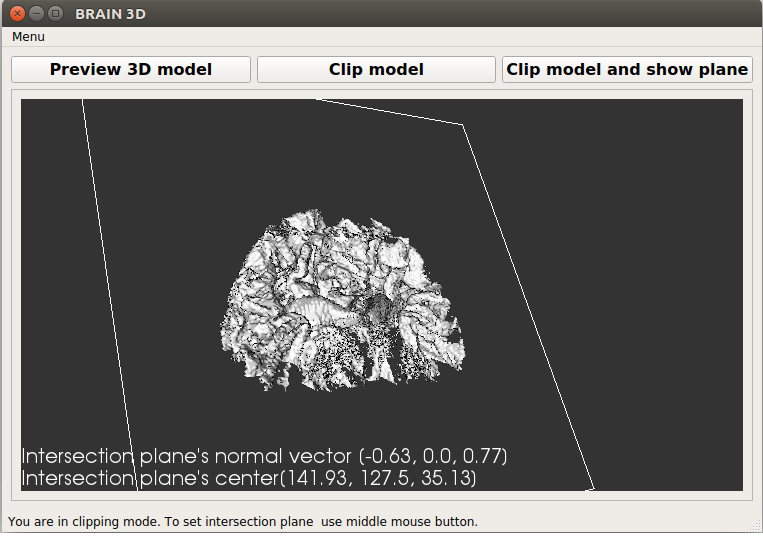
\includegraphics[scale=0.7]{figures/Module_11/11_test_7.png}\caption{Clipped model in elected plane. \label{fig:figures/11_test_7}}
\end{figure}

\begin{figure}[H]
\centering{}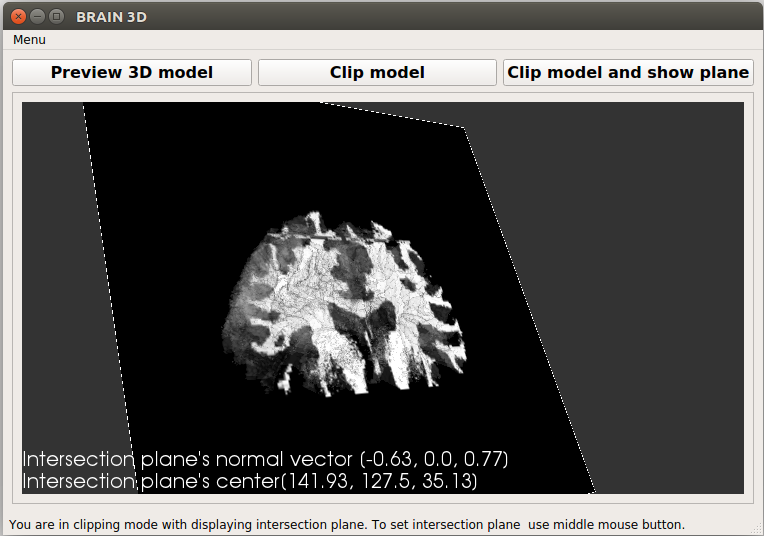
\includegraphics[scale=0.7]{figures/Module_11/11_test_8.png}\caption{Clipped model in the same elected plane with cross-intersection image. \label{fig:figures/11_test_8}}
\end{figure}


\indent In menu user has option to display help window with short user guide. \ref{fig:figures/11_help}
\begin{figure}[H]
\centering{}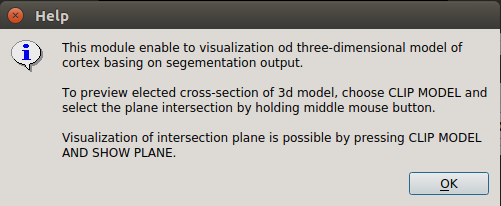
\includegraphics[scale=0.7]{figures/Module_11/11_help.png}\caption{Help window with short user guide. \label{fig:figures/11_help}}
\end{figure}

\indent Automatically tests are also implemented. Unit tests cover the verification of  input data and output of reconstruction function. There are three test cases:


\begin{enumerate}
\item \textbf{test invalid input data format} - checking if program raises error when the input data contains empty segementation parameter of main class. 
\item \textbf{test invalid input data type} - checking if program raises error when the input data contains array in inappropriate dimension as segementation parameter of main class.
\item \textbf{test generate model} - checking if function returns object of vtkImageData and vtkPolyData type.
\end{enumerate}
\begin{figure}[H]
\centering{}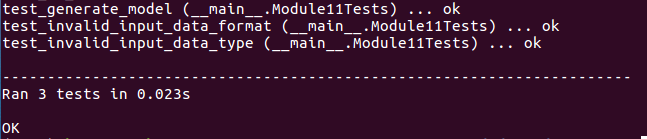
\includegraphics[scale=0.7]{figures/Module_11/11_unit_test.png}\caption{Result of unit tests. \label{fig:figures/11_unit_test}}
\end{figure}




